\setcounter{section}{1}

\section{Лексичний аналіз та скінченні автомати}

\subsection{Лексичний аналіз в мовних процесорах}

\textbf{Призначення:} перетворення вхідного тексту програми з формату зовнішнього представлення в машинно-орієнтований формат --- послідовність лексем. \medskip

Нагадаємо, що \textit{лексема} --- це ланцюжок літер елементарний об'єкт програми, що несе певний семантичний зміст. В подальшому кожну лексему будемо представляти як пару $\langle\text{клас лексеми}, \text{ім'я лексеми}\rangle$. \medskip

В більшості мов програмування для визначення класів лексем достатньо скінчених автоматів.

\subsection{Скінчені автомати}

\textit{Недетермінований скінчений автомат} --- це п'ятірка $M = \left\langle Q, \Sigma, \delta, q_0, F \right\rangle$, де
\begin{itemize}
	\item $Q = \{q_0, q_1, \ldots, q_{n-1}\}$ --- скінчена множина станів автомата;
	\item $\Sigma = \{a_1, a_2, \ldots, a_m\}$ --- скінчена множина вхідних символів (вхідний \textit{алфавіт});
	\item $q_0 \in Q$ --- \textit{початковий} стан автомата;
	\item $\delta$ --- відображення множини $Q \times \Sigma$ в множину $2^Q$. Відображення $\delta$ як правило називають \textit{функцією переходів};
	\item $F \subset Q$ --- множина заключних станів. Елементи з $F$ називають \textit{заключними} або \textit{фінальними} станами.
\end{itemize}

Якщо $M$ --- скінчений автомат, то пара $(q, w) \in Q \times \Sigma^\star$ називається \textit{конфігурацією} автомата $M$. Оскільки скінчений автомат --- це дискретний пристрій, він працює по тактам. \textit{Такт} скінченого автомата $M$ задається бінарним відношенням $\models$, яке визначається на конфігураціях:
\begin{equation}
	(q_1, a w) \models (q_2, w) \quad \text{if} \quad q_2 \in \delta(q_1, a), \quad \forall w \in \Sigma^\star.
\end{equation}

\subsubsection{Мова яку розпізнає скінченний автомат}

Скінченний автомат $M$ \textit{розпізнає (допускає)} ланцюжок $w$, якщо
\begin{equation}
	\exists q \in F: \quad (q_0, w) \models^\star (q, \varepsilon),
\end{equation}
де $\models^\star$ --- рефлексивно-транзитивне замикання бінарного відношення $\models$. \medskip

\textit{Mова}, яку допускає автомат $M$ (розпізнає автомат $M$)
\begin{equation}
	L(M) = \{w \mid w \in \Sigma^\star, \exists q \in F: (q_0, w) \models^\star (q, \varepsilon)\}.
\end{equation}

\subsubsection{Способи визначення функції переходів}

На практиці, при визначенні скінченого автомата $M$, використовують декілька способів визначення функції $\delta$, наприклад: 
\begin{itemize}
	\item це табличне визначення $\delta$;
	\item діаграма проходів скінченого автомата.
\end{itemize}

\textit{Табличне визначення} функції $\delta$ --- це таблиця $M(q_i, a_j)$, де $a_j \in \Sigma, q_i \in Q$, тобто
\begin{equation}
	M(q_i, a_j) = \{ q_k \mid q_k \in \delta(q_i, a_j) \}.
\end{equation}

\textit{Діаграма переходів} скінченого автомата $M$ --- це невпорядкований граф $G(V, P)$, де $V$ --- множина вершин графа, а $P$ --- множина орієнтованих дуг, причому з вершини $q_i$ у вершину $q_j$ веде дуга позначена $a_k$, коли $q_j \in \delta(q_i, a_k)$. На діаграмі переходів скінченого автомата це позначається так:
\begin{figure}[H]
	\centering
	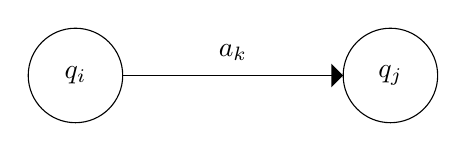
\begin{tikzpicture}[scale=0.2]
\tikzstyle{every node}+=[inner sep=0pt]
\draw [black] (0,0) circle (3);
\draw (0,0) node {$q_i$};
\draw [black] (20,0) circle (3);
\draw (20,0) node {$q_j$};
\draw [black] (3,0) -- (17,0);
\fill [black] (16.25,.75) -- (17,0) -- (16.25,-.75);
\draw (10,2) node [below] {$a_k$};
\end{tikzpicture}

\end{figure}

В подальшому, на діаграмі переходів скінченого автомата $M$ елементи з множини заключних станів будемо позначити так:
\begin{figure}[H]
	\centering
	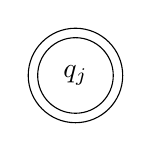
\begin{tikzpicture}[scale=0.2]
\tikzstyle{every node}+=[inner sep=0pt]
\draw [black] (0,0) circle (3);
\draw (0,0) node {$q_j$};
\draw [black] (0,0) circle (2.4);
\end{tikzpicture}

\end{figure}

\textbf{Приклад.} Побудуємо діаграму переходів скінченого автомата $M$, який розпізнає множину цілочислових констант мови С.
\begin{figure}[H]
	\centering
	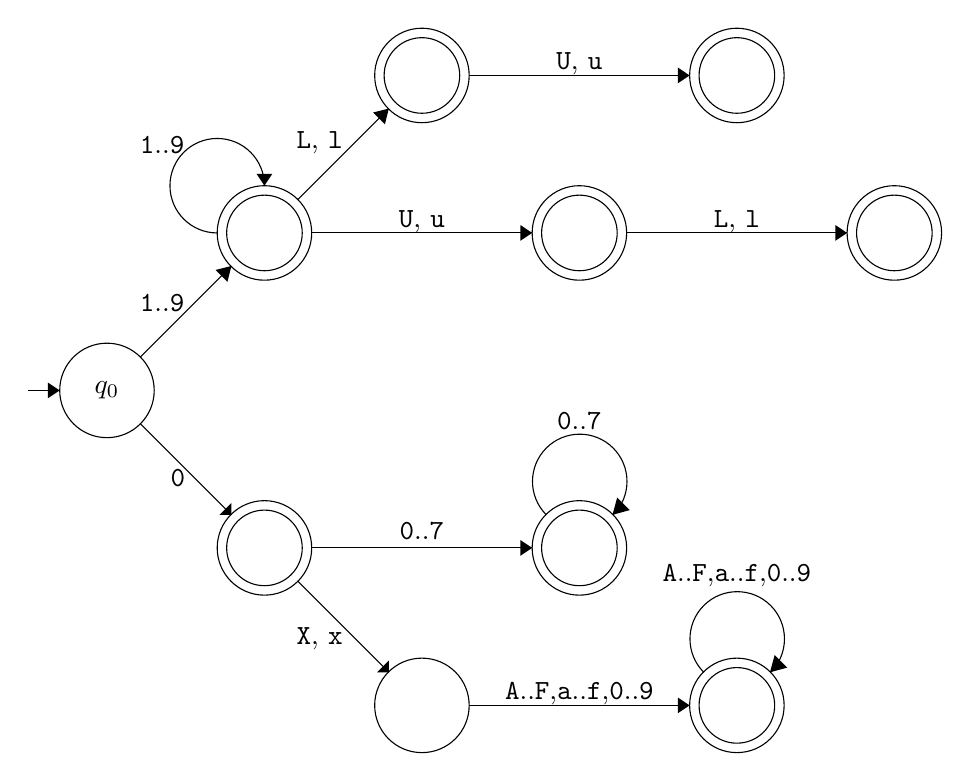
\begin{tikzpicture}[scale=0.2]
\tikzstyle{every node}+=[inner sep=0pt]
\draw [black] (-5,0) -- (-3,0);
\fill [black] (-3,0) -- (-3.75,-.5) -- (-3.75,.5);
\draw [black] (0,0) circle (3);
\draw (0,0) node {$q_0$};

\draw [black] (2.1, 2.1) -- (7.9,7.9);
\fill [black] (6.9,7.65) -- (7.9,7.9) -- (7.65,6.9);
\draw (3.5,5) node [above] {{\tt1}..{\tt9}};
\draw [black] (10,10) circle (3);
\draw [black] (10,10) circle (2.4);
\draw (3.5,15) node [above] {{\tt1}..{\tt9}};
\draw [black] (7,10) arc (270:0:3);
\fill [black] (10,13) -- (10.5,13.75) -- (9.5,13.75);

\draw [black] (2.1, -2.1) -- (7.9,-7.9);
\fill [black] (7.15,-7.9) -- (7.9,-7.9) -- (7.9,-7.15);
\draw (4.5,-5) node [below] {{\tt0}};
\draw [black] (10,-10) circle (3);
\draw [black] (10,-10) circle (2.4);

\draw [black] (12.1, 12.1) -- (17.9,17.9);
\fill [black] (16.9,17.65) -- (17.9,17.9) -- (17.65,16.9);
\draw (13.5,15) node [above] {{\tt L}, {\tt l}};
\draw [black] (20,20) circle (3);
\draw [black] (20,20) circle (2.4);

\draw [black] (13,10) -- (27,10);
\fill [black] (27,10) -- (26.25,9.5) -- (26.26,10.5);
\draw (20,10) node [above] {{\tt U}, {\tt u}};
\draw [black] (30,10) circle (3);
\draw [black] (30,10) circle (2.4);

\draw [black] (23,20) -- (37,20);
\fill [black] (37,20) -- (36.25,19.5) -- (36.26,20.5);
\draw (30,20) node [above] {{\tt U}, {\tt u}};
\draw [black] (40,20) circle (3);
\draw [black] (40,20) circle (2.4);

\draw [black] (33,10) -- (47,10);
\fill [black] (47,10) -- (46.25,9.5) -- (46.26,10.5);
\draw (40,10) node [above] {{\tt L}, {\tt l}};
\draw [black] (50,10) circle (3);
\draw [black] (50,10) circle (2.4);

\draw [black] (13,-10) -- (27,-10);
\fill [black] (26.25,-10.5) -- (26.25,-9.5) -- (27,-10);
\draw (20,-9.5) node [above] {{\tt0}..{\tt7}};
\draw [black] (30,-10) circle(3);
\draw [black] (30,-10) circle (2.4);
\draw (30,-2.5) node [above] {{\tt0}..{\tt7}};
\draw [black] (27.9,-7.9) arc (225:-45:3);
\fill [black] (32.1,-7.9) -- (32.4,-6.8) -- (33.2,-7.6);

% \draw [black] (2.1+10, 2.1-10) -- (7.9+10,7.9-10);
% \fill [black] (6.9+10,7.65-10) -- (7.9+10,7.9-10) -- (7.65+10,6.9-10);
% \draw (3.5+10,5-10) node [above] {{\tt0}..{\tt7}};
% \draw [black] (10+10,10-10) circle (3);
% \draw [black] (10+10,10-10) circle (2.4);
% \draw (3.5+10,15-10) node [above] {{\tt0}..{\tt7}};
% \draw [black] (7+10,10-10) arc (270:0:3);
% \fill [black] (10+10,13-10) -- (10.5+10,13.75-10) -- (9.5+10,13.75-10);

\draw [black] (12.1, -12.1) -- (17.9,-17.9);
\fill [black] (17.15,-17.9) -- (17.9,-17.9) -- (17.9,-17.15);
\draw (13.5,-15) node [below] {{\tt X}, {\tt x}};
\draw [black] (20,-20) circle (3);

\draw [black] (23,-20) -- (37,-20);
\fill [black] (36.25,-20.5) -- (36.25,-19.5) -- (37,-20);
\draw (30,-20) node [above] {{\tt A}..{\tt F},{\tt a}..{\tt f},{\tt0}..{\tt9}};
\draw [black] (40,-20) circle(3);
\draw [black] (40,-20) circle (2.4);
\draw (10+30,17.5-30) node [above] {{\tt A}..{\tt F},{\tt a}..{\tt f},{\tt0}..{\tt9}};
\draw [black] (7.9+30,12.1-30) arc (225:-45:3);
\fill [black] (12.1+30,12.1-30) -- (12.4+30,13.2-30) -- (13.2+30,12.4-30);
\end{tikzpicture}

\end{figure}

\textbf{Зауваження.} Цей автомат неповний, на два нижні праві вузли потрібно довісити ``UL''-частину яка висить на вузлі ``1..9''. \medskip

З побудованого прикладу видно, що приведений автомат не повністю визначений.

\subsubsection{Детерміновані скінченні автомати}

Скінчений автомат $M$ називається \textit{детермінованим}, якщо $\delta(a_i, a_k)$ містить не більше одного стану для любого $q_i \in Q$ та $a_k \in \Sigma$. \medskip

\textbf{Теорема.} \textit{Для довільного недетермінованого скінченого автомата $M$ можна побудувати еквівалентний йому детермінований скінчений автомат $M'$, такий що $L(M) = L(M')$.} \medskip


\textbf{Доведення:} Нехай $M$ --- недетермінований скінчений автомат \[M = \langle Q, \Sigma, \delta, q_0, F\rangle. \]

Детермінований автомат $M' = \langle Q', \Sigma, \delta', q_0', F\rangle$ побудуємо таким чином:
\begin{enumerate}
	\item $Q' = 2^Q$, тобто імена станів автомата $M'$ --- це підмножини множини $Q$.
	\item $q_0' = \{q_0\} \in 2^Q = Q'$.
	\item $F'$ складається з усіх таких підмножин $S \in 2^Q = Q'$, що $S \cap F \ne \varnothing$.
	\item $\delta'(S, a) \models \{q \mid q \in \delta(q_i, a), q_i \in S\}$.
\end{enumerate}

Доводимо індукцією по $i$, що $(S, w) \models^i (S', \varepsilon)$, тоді і тільки тоді, коли $S' = \{q \mid \exists q_i \in S: (q_i, w) \models^i (q, \varepsilon)\}$. \medskip

Зокрема, $ (\{q_0\}, w) \models^\star (S', \varepsilon)$, для деякого $S' \in F'$, тоді і тільки тоді, коли $\exists q \in F: (q_0, w) \models^\star (q, \varepsilon)$. \medskip

Таким чином, $L(M) = L(M')$. \medskip

Побудований нами автомат $M$ має дві властивості: він детермінований та повністю визначений. До того ж кількість станів цього автомата $2^n - 1$.

\subsection{Контрольні запитання}

\begin{enumerate}
	\item У чому призначення лексичного аналізу? % перетворення вхідного тексту програми з формату зовнішнього представлення в послідовність лексем.
	\item Що таке недетермінований скінчений автомат? % п'ятірка (стани, алфавіт, початковий стан, заключні стани, функція переходів)
	\item Яку мову розпізнає скінченний автомат? % всі слова що переводять автомат з початкового стану у заключний
	\item Які два способи визначення функції переходів ви знаєте? % табличне і через діаграму переходів
	\item Спробуйте ``зламати'' вищенаведений автомат для цілочислових констант мови C (зверніть увагу на зауваження). % ll, LL?
	\item Що таке детермінований скінчений автомат? % скінченний автомат з однозначною функцією переходів
	\item Сформулюйте і доведіть теорему про детермінізацію скінченного автомата.
	\item Нехай функція переходів $\delta$ не однозначна, але у той же час набуває не багато різних значень на одному наборі аргументів, наприклад не більше двох, тобто $|M(q, a)| \le 2$ для довільних $q \in Q$ і $a \in \Sigma$. Чи можна тоді отримати кращу оцінку зверху на кількість станів еквівалентного детермінованого автомату ніж $2^n - 1$?
\end{enumerate}
